\documentclass{sig-alternate-2013}

\usepackage{multirow}
\usepackage{eurosym}
\usepackage{caption}
\usepackage{url}
\usepackage[draft,inline,nomargin]{fixme}
\usepackage{hyperref}
\usepackage{subfig} 
\usepackage{paralist}
\usepackage[tracking=true]{microtype}
\usepackage{todonotes}

\newcommand{\superscript}[1]{\ensuremath{^{\textrm{#1}}}}
\def\sharedaffiliation{\end{tabular}\newline\begin{tabular}{c}}

\def\wu{\superscript{*}}
\def\wg{\superscript{\dag}}
\def\wh{\superscript{\ddag}}

\hyphenation{Rijksmuseum}
\hyphenation{CrowdFlower}


\newfont{\mycrnotice}{ptmr8t at 7pt}
\newfont{\myconfname}{ptmri8t at 7pt}
\let\crnotice\mycrnotice%
\let\confname\myconfname%

\permission{Permission to make digital or hard copies of part or all of this work for personal or classroom use is granted without fee provided that copies are not made or distributed for profit or commercial advantage, and that copies bear this notice and the full citation on the first page. Copyrights for third-party components of this work must be honoured. For all other uses, contact the owner/author(s). Copyright is held by the author/owner(s).}
\conferenceinfo{WebSci'14,}{June 23--26, 2014, Bloomington, IN, USA.} 
\copyrightetc{ACM \the\acmcopyr}
\crdata{978-1-4503-2622-3/14/06. \\
http://dx.doi.org/10.1145/2615569.2615644}

\clubpenalty=10000 
\widowpenalty = 10000

\fxsetup{theme=color,mode=multiuser, }

\begin{document}

\title{Crowdsourcing Knowledge-Intensive Tasks \\In Cultural Heritage}

\subtitle{\large\textbf{{Jasper~Oosterman\wu, Archana~Nottamkandath\wg, Chris~Dijkshoorn\wg, Alessandro~Bozzon\wu, Geert-Jan~Houben\wu, Lora~Aroyo\wg}}}
%

\numberofauthors{3}
\author{
% 1st. author
\alignauthor 
       \affaddr{{\wu}Delft University of Technology} \\
       \affaddr{Web Information Systems} \\
       \affaddr{P.O. Box 5, 2600 AA} \\
       \affaddr{Delft, The Netherlands} \\
       \email{\small{\{j.e.g.oosterman,a.bozzon,\\g.j.p.m.houben\}@tudelft.nl}}
\and
% 2nd. author
\alignauthor 
       \affaddr{{\wg}VU University Amsterdam} \\
       \affaddr{De Boelelaan 1081a} \\
       \affaddr{1081 HV Amsterdam} \\
       \affaddr{Amsterdam, The Netherlands} \\
       \email{\small{\{a.nottamkandath,c.r.dijkshoorn,\\lora.aroyo\}@vu.nl}}       
}

\maketitle   
       
\begin{abstract}
Large datasets such as Cultural Heritage collections require detailed annotations when digitised and made available online. Annotating different aspects of such collections requires a variety of knowledge and expertise which is not always possessed by the collection curators.
Artwork annotation is an example of a \emph{knowledge intensive} image annotation task, i.e. a task that demands annotators to have domain-specific knowledge in order to be successfully completed.
%People with the right domain knowledge need to be found and engaged to contribute their knowledge to these knowledge intensive tasks.
This paper describes the results of a study aimed at investigating the applicability of crowdsourcing techniques to \emph{knowledge intensive} image annotation tasks. We observed a clear relationship between the annotation difficulty of an image, in terms of number of items to identify and annotate, and the performance of the recruited workers. 

%  on the designed and performed an experiment involving the prints collection of the Rijksmuseum Amsterdam, and we 
%involving both experts and crowd workers in the domain-specific description of depicted flowers. Our work contributes with novel findings on how generic crowd workers can provide meaningful contribution to artwork annotation with domain-specific knowledge. We show that crowd workers can provide performance comparable to experts for a range of \emph{knowledge intensive} image annotations.
\end{abstract}

\category{H.4}{Information Systems Applications}{Miscellaneous}
\keywords{Crowdsourcing; Cultural Heritage; Knowledge Intensive Tasks}

\section{Introduction}
Some crowdsourcing tasks, referred to as \emph{knowledge intensive tasks}\cite{Oosterman:2014}, require specific knowledge to be successfully executed. An example is the annotation of flower images with the correct botanical names. Typically, cultural heritage institutions employ professionals, mostly art historians, who provide excellent annotations about the art-historical aspects of artworks, but lack domain expertise for other aspects such as the name of the depicted flowers. For these other aspects, people with the right domain expertise need to be found and engaged, a process called nichesourcing~\cite{Boer2012}. How to do nichesourcing effectively is an emerging research area. 

Image annotation tasks require annotators to provide tags that describe the presence of one or more instance of a given generic entity (e.g. flowers, birds, etc.). This class of tasks is typically performed on photographic images, which carefully represent the real world; they are also quickly performed, as the knowledge and skills required for their execution are commonly available in the general population (e.g. the ability to recognise a flower). We claim the annotation of artworks to be a more involved process, especially when coupled with the need for accurate, possibly domain-specific labels. It is a good example of  a \textit{knowledge intensive} image annotation task, that features \textit{entity identification} as an important source of complexity. The correct recognition of the targeted entities in an art image might be hindered by its artistic representation; for instance, colours or details might be missing; or the depicted content might be stylised or even completely abstract. This additional complexity increases the cognitive effort for an annotator by needing to 1) have the ability to ``see'' the raw content trough the lens of a given style or technique; and 2) possess domain-specific knowledge. 

In a previous work\cite{Oosterman:2014} we showed that niche sourcing can help with the creation of useful annotations in the domain of cultural heritage. In this paper, we study the performance of workers employed via crowdsourcing platforms for annotating a collection of prints depicting flowers from the Rijksmuseum Amsterdam\footnote{\url{http://rijksmuseum.nl}}. We have created a testbed, similar to existing image annotation interfaces, where workers could tag prints with the specific names of flowers. The testbed measured the annotation behaviour of the workers and stored the annotations. In our study we try to answer the following questions: \emph{What is the relation between entity identification difficulty and crowd annotation behaviour?}


\section{Experimental Setup}

\begin{figure*}[ht]
      \centering
      \subfloat[Workers Precision\label{fig:precbycountry}]{
	  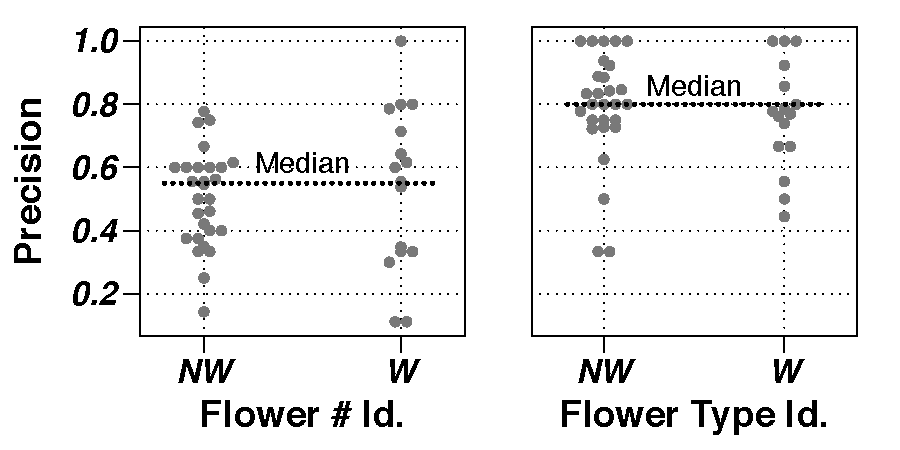
\includegraphics[width=0.30\textwidth]{figures/numbersByCountry2.pdf}
      }
      \quad
      \subfloat[Workers Error Rate\label{fig:errordiff}]{
	  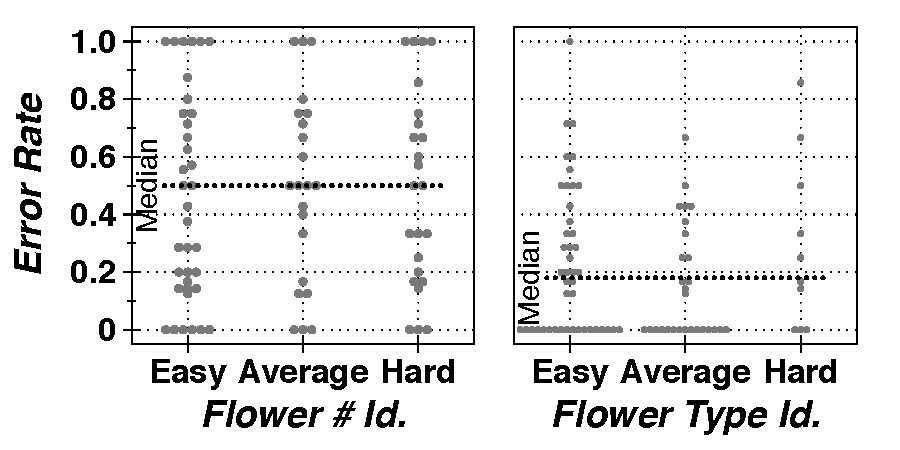
\includegraphics[width=0.30\textwidth]{figures/identificationQualityDiffPoints.pdf}
      }
      \quad
      \subfloat[Workers Error Rate\label{fig:errorpnp}]{
	  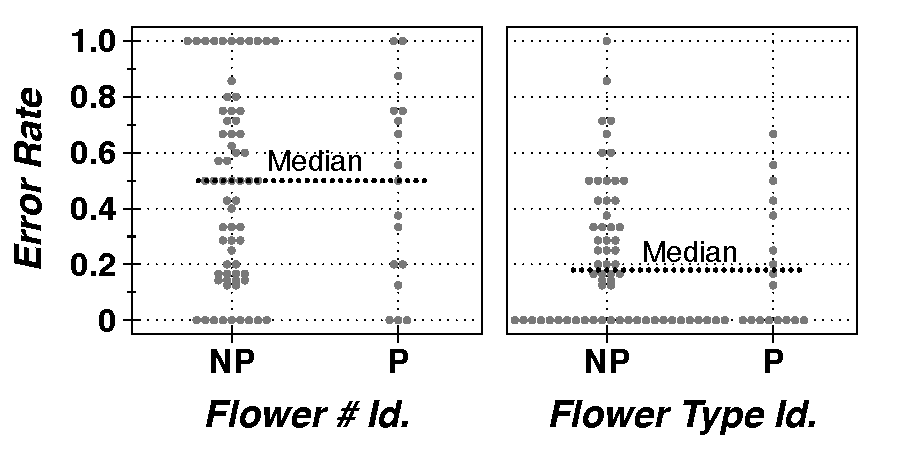
\includegraphics[width=0.30\textwidth]{figures/identificationQualityPNPPoints.pdf}
      }
  \caption{Distribution of worker precision w.r.t to identification difficulty and prominence}\label{fig:workerscountrystat}
\end{figure*}


We manually selected 82 prints that were annotated with the \textit{Flowers} taxonomy term, i.e. prints that were identified as containing at least one flower. A team of 3 trusted annotators inspected each print, labelling it as \textbf{Prominent (P)} ($17$ prints) or \textbf{Non Prominent (NP)} ($65$ prints), counting the number of contained \textbf{flower instances}, and counting the number of \textbf{flower types}. 
Despite the full focus and attention put in this annotation process, some prints proved challenging to label. To account for such difficulty, we classify prints in three categories, according to the \textit{disagreement} shown by the trusted annotators when counting the number of identified flower instances and flower types. Respectively: \textbf{Easy}: prints where all trusted annotators agreed on the same count; \textbf{Average}: prints where trusted annotators disagreed by 1 or 2 flowers/types; \textbf{Hard}: prints where the trusted annotators disagreed by more than 3 flowers/types. Table \ref{tab:taskdifficulty} reports the distribution of number of prints according to their combined identification difficulty. %There is a positive correlation between the difficulty in flower instances identification and flower types identification. %Interestingly, the identification of flower \textit{types} was perceived by our trusted assessors in general as easier than the identification of flower \textit{instances}.

\begin{table}
\small
	\centering
	\setlength{\tabcolsep}{2pt}
	\renewcommand{\arraystretch}{1.1}
	\begin{tabular}{ll | c | c | c | c }
	\cline{3-5}
	&			 		& \multicolumn{3}{c|}{Flower Type} & \\  \cline{3-6}
	&		 			& \textbf{Easy}	& \textbf{Average}	& \textbf{Hard} & \multicolumn{1}{||c|}{\textbf{\textit{Total}}}\\  \hline
	\multicolumn{1}{|c|}{\multirow{3}{*}{\rotatebox{270}{\shortstack{\hspace{-12px}Flower \\ \hspace{-8px}Number}}}} & \textbf{Easy}  		& 30 				& 6	 				& 0 & \multicolumn{1}{||c|}{\textbf{36}}\\  \cline{2-6}
	\multicolumn{1}{|c|}{}& \textbf{Average} 	& 10				& 11 				& 1 & \multicolumn{1}{||c|}{\textbf{22}} \\  \cline{2-6}
	\multicolumn{1}{|c|}{}& \textbf{Hard}	& 4 				& 11 				& 9 & \multicolumn{1}{||c|}{\textbf{24}} \\ \hline\cline{2-6}
			\multicolumn{1}{c|}{}			& \textbf{\textit{Total}}	& \textbf{44} 				& \textbf{28} 				& \textbf{10} & \multicolumn{1}{||c|}{\textbf{82}} \\ \cline{2-6}

	\end{tabular}
	\caption{Distribution of prints in the dataset according to the assessed entity identification difficulty.}
	\label{tab:taskdifficulty}
\end{table}

The experiment was performed in February 2014, and it involved anonymous annotators drawn from the \textit{CrowdFlower}\footnote{\url{http://crowdflower.com}} platform, which recruits workers worldwide. Of 732 workers that inspected the published task, 151 attempted execution (abandonment rate of 80\%), and only 44 passed the qualification test and the designed quality checks. An extended description of the experimental setup and the resulting data is available online\footnote{\url{http://www.wis.ewi.tudelft.nl/WebScience2014}}.

Each print annotation required workers to indicate the number of flower instances, and the number of flower types they were able to identify. We compared the provided numbers with the corresponding assessment performed by our trusted annotators. With \texttt{easy} prints, we considered correct only values equal to the ground-truth ones. With \texttt{average} and \texttt{hard} prints, we considered correct values falling in the range of disagreement of the trusted annotators. Figure \ref{fig:precbycountry} reports the average precision of workers, aggregated according to the country of belonging (Western --  Western Europe, plus USA and Canada -- and non-western). Figure \ref{fig:errordiff} and Figure \ref{fig:errorpnp} depicts the average error rate of workers according to the flower identification difficulty and to the flower prominence on the print. Flower type identification is generally performed more precisely than flower number identification, although hard and non-prominent prints generally lead to more errors. Flower type identification was also performed more precisely by Western workers, but errors affect every category of prints in a similarly distributed manner.

\section{Discussion and Conclusion}

Our study provided interesting insights on the nature of the annotation behaviour of crowd workers in knowledge-intensive image annotation tasks. With respect to our research question, we observed that the difficulty in flower identification clearly played a role in the performance of workers. Tasks addressing difficult prints achieved, on average, a worse flower number identification precision. This result can be explained by the nature of the flower number identification task, which is tedious and very error-prone: the very high abandonment rate at task inspection (80\%) combined with the comparably relevant number of low quality workers suggests the adoption of a different task design. For instance, a more structured task decomposition (e.g. showing just a portion of the print), or more engaging and/or rewarding interactions (e.g. using a game with a purpose) could result in better performance. Studies about the adoption of such solutions are planned for future work. Flower type identification, compared to flower instance identification, generally resulted in a lower error rate, thus suggesting that anonymous crowd workers can effectively support this aspect of knowledge intensive image annotation tasks. Prints with prominent flowers received on average a slightly bigger number of tags. In future work, we will continue our investigation on the targeted dataset, including an analysis of the quality of the retrieved annotations. We also plan investigations addressing other knowledge domains  (e.g. annotation of birds, castles, etc.). We will also focus on user modelling and expert finding \cite{bozzon2013} in the crowd such that given a task pre-selected contributors can be contacted (nichesourcing)\cite{Boer2012}.

\vspace{5px}
\noindent\textbf{Acknowledgements}. This publication was supported by the Dutch national program COMMIT.
%\bibliographystyle{abbrv}
\bibliographystyle{unsrt}
\bibliography{literature} 
\balancecolumns

\end{document}
